%%%%%%%%%%%%%%%%%%%%%%%%%%%%%%%%%%%%%%%%%%%%%%%%%%%%%%
% A Beamer template for University of Wollongong     %
% Based on THU beamer theme                          %
% Author: Qiuyu Lu                                   %
% Date: July 2024                                    %
% LPPL Licensed.                                     %
%%%%%%%%%%%%%%%%%%%%%%%%%%%%%%%%%%%%%%%%%%%%%%%%%%%%%%
% Customized for Sharif University of Technology     %
%%%%%%%%%%%%%%%%%%%%%%%%%%%%%%%%%%%%%%%%%%%%%%%%%%%%%%


\documentclass[serif, aspectratio=169]{beamer}
\usepackage{pgfplots} % Required for plotting
\pgfplotsset{compat=1.17} % Compatibility level
%\documentclass[serif]{beamer}  % for 4:3 ratio
\usepackage[T1]{fontenc} 
\usepackage{fourier} % see "http://faq.ktug.org/wiki/uploads/MathFonts.pdf" for other options
\usepackage{hyperref}
\usepackage{latexsym,amsmath,xcolor,multicol,booktabs,calligra}
\usepackage{graphicx,pstricks,listings,stackengine}
\usepackage{lipsum}
\usepackage{array}

\author{Ali Sharifi-Zarchi}
\title{Machine Learning (CE 40477)}
\subtitle{Fall 2024}
\institute{
    CE Department \\
    Sharif University of Technology
}
%\date{\small \today}
% \usepackage{UoWstyle}
\usepackage{SUTstyle}

% defs
\def\cmd#1{\texttt{\color{red}\footnotesize $\backslash$#1}}
\def\env#1{\texttt{\color{blue}\footnotesize #1}}
\definecolor{deepblue}{rgb}{0,0,0.5}
\definecolor{deepred}{RGB}{153,0,0}
\definecolor{deepgreen}{rgb}{0,0.5,0}
\definecolor{halfgray}{gray}{0.55}

\lstset{
    basicstyle=\ttfamily\small,
    keywordstyle=\bfseries\color{deepblue},
    emphstyle=\ttfamily\color{deepred},    % Custom highlighting style
    stringstyle=\color{deepgreen},
    numbers=left,
    numberstyle=\small\color{halfgray},
    rulesepcolor=\color{red!20!green!20!blue!20},
    frame=shadowbox,
}


\begin{document}

\begin{frame}
    \titlepage
    \vspace*{-0.6cm}
    \begin{figure}[htpb]
        \begin{center}
            
\includegraphics[keepaspectratio, scale=0.25]{pic/sharif-main-logo.png}
        \end{center}
    \end{figure}
\end{frame}

\begin{frame}    
\tableofcontents[sectionstyle=show,
subsectionstyle=show/shaded/hide,
subsubsectionstyle=show/shaded/hide]
\end{frame}

\section{Regularization \& Overfitting}

\subsection{Reviewing the Problem of Overfitting}

\begin{frame}{Reviewing the Problem of Overfitting}
    \begin{itemize} 
    
        \item \textbf{Recall from previous lectures:} Overfitting vs Underfitting
        
        \item \textbf{Overfitting:} Learning the underlying patterns and noise in the training data.
        \begin{itemize}
            \item High accuracy on training data but poor generalization on unseen data.
        \end{itemize}  

        \item \textbf{Underfitting:} The model is too simple to capture the patterns in the data.
        \begin{itemize}
            \item Poor performance on both training and test data.
        \end{itemize}

        \begin{figure}
                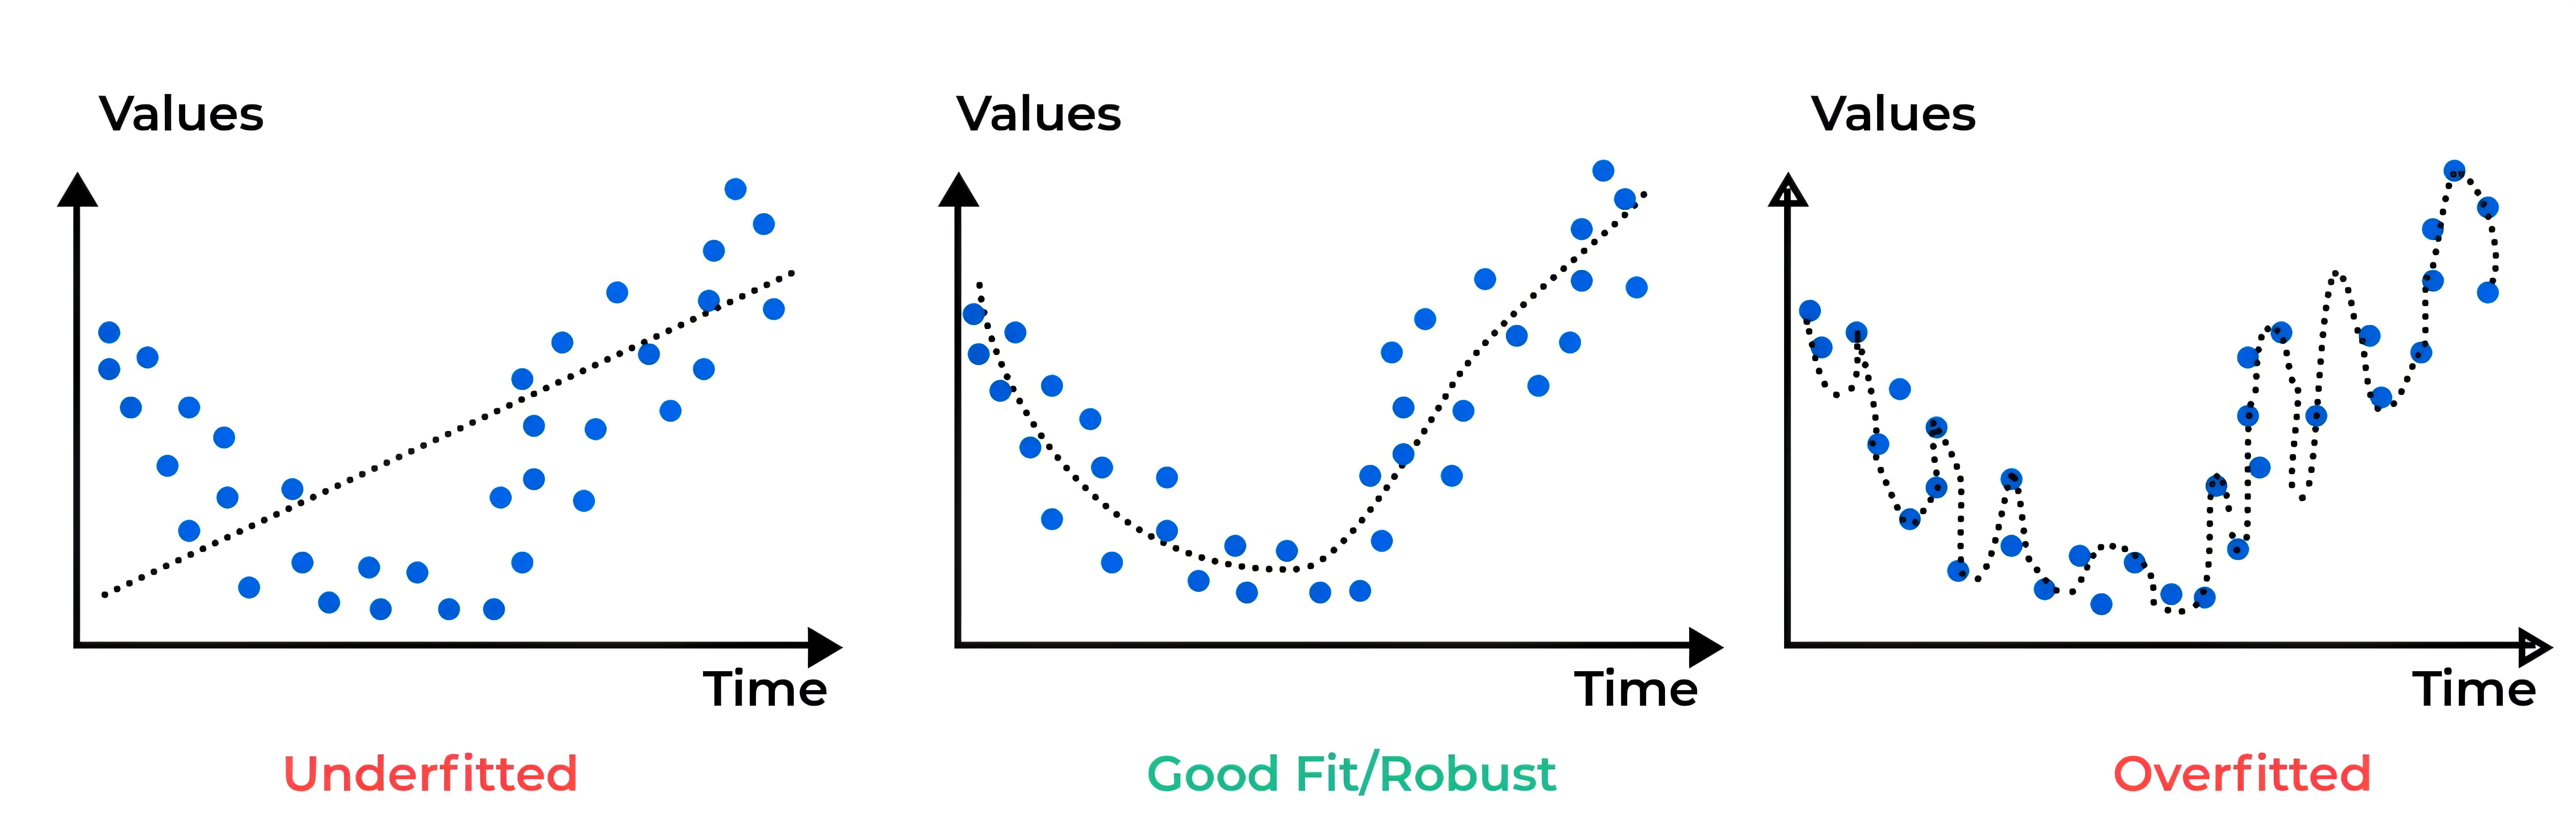
\includegraphics[width=0.85\textwidth]{pic/overfitting-vs-underfitting__AIE.png}
                \label{fig:overfitting-vs-underfitting}
                \caption{\href{https://analystprep.com/study-notes/cfa-level-2/quantitative-method/overfitting-methods-addressing/}{\textcolor{orange}{\textbf{Source}}}}
        \end{figure}

    \end{itemize} 
\end{frame}

\subsection{Regularization in Neural Networks}

\begin{frame}{Regularization in Neural Networks}
        \begin{itemize}
            \item \textbf{Goal:} Prevent overfitting.
            \item \textbf{Key Idea:} Favor simpler models to avoid fitting noise in the data.
        \end{itemize}

    \begin{figure}
        \centering
        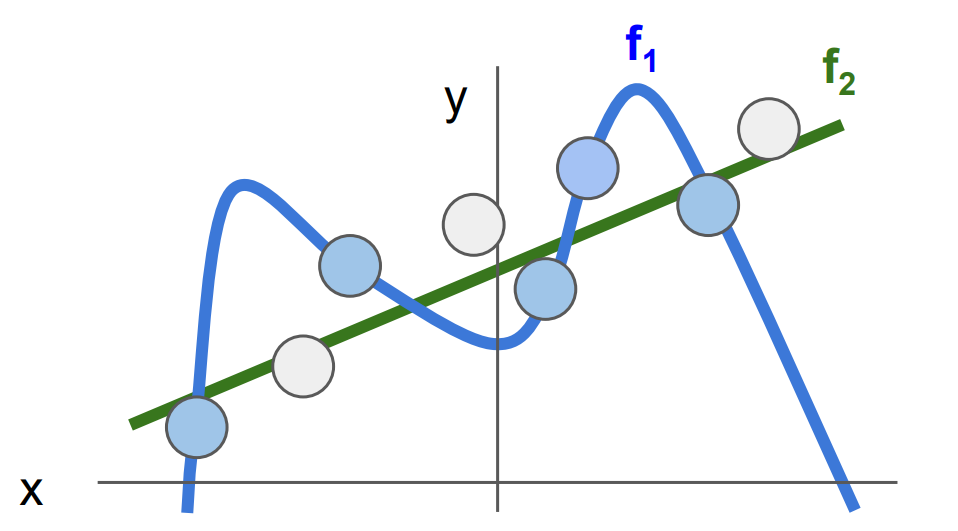
\includegraphics[width=0.5\textwidth]{pic/Regularization-intuition.png}
        \caption{Regularization prevents overfitting by avoiding fitting noise in the data [1].}
        \label{fig:Regularization-intuition}
    \end{figure}
\end{frame}


\begin{frame}{Regularization in Neural Networks}
    
\begin{equation}
J_\lambda(w) = \underbrace{J(w)}_{{\substack{\vphantom{\text{Prevent the model}} \\ \text{\textcolor{green} {\textbf{Data loss}}: Model predictions} \\ \text{should match training data}}}} + \underbrace{\lambda R(w)}_{{\substack{\vphantom{\text{Prevent the model}} \\ \text{\textcolor{green} {\textbf{Regularization}}: Prevent the model} \\ \text{from doing \textit{too} well on training data}}}}
\end{equation}


\end{frame}

\subsection{Key Regularization Techniques}
\begin{frame}{Key Regularization Techniques}
    \begin{itemize}[<+-| alert@+>] % stepwise alerts

            \item L1 (Lasso): Sparse weights, feature selection
                \begin{equation}
                    \text{L1 Regularization} = \lambda \sum_{j=1}^{m} |w_j|
                \end{equation}

            \item L2 (Ridge): Adds a penalty for large weights to the loss function
                \begin{equation}
                    \text{L2 Regularization} = \lambda \sum_{j=1}^{m} w_j^2 =
                    \lambda \textbf{W}^T\textbf{W}
                \end{equation}

            \item Elastic Net (L1 + L2): Combines both L1 and L2 penalties, where $\beta$ controls the balance between L1 and L2 regularization.

                \begin{equation}
                    \text{Elastic net Regularization} =\lambda \sum_{j=1}^{m} (\beta|w_j| + \frac{1-\beta}{2} w_j^2)
                \end{equation}
            
    \end{itemize}
\end{frame}

\begin{frame}{Key Regularization Techniques}

            \begin{figure}
                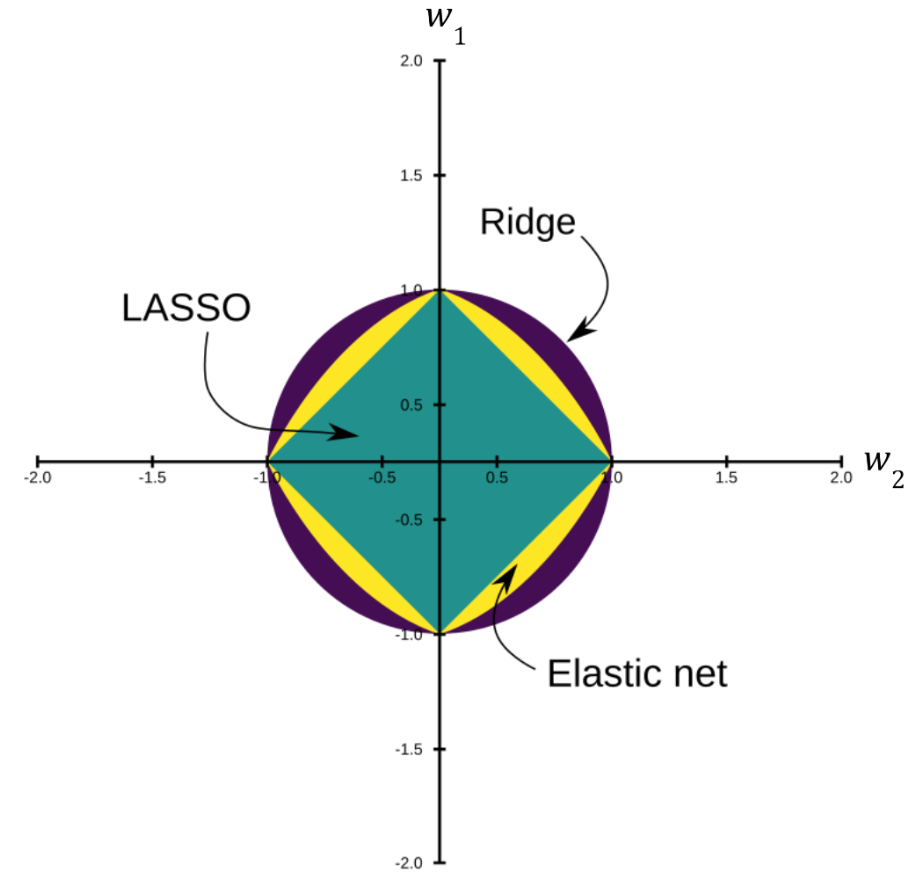
\includegraphics[width=0.4\textwidth]{pic/Regularization.png}
                 \caption{Lasso, Ridge, and Elastic net Comparision. \href{https://analyticsindiamag.com/ai-mysteries/hands-on-tutorial-on-elasticnet-regression/}{\textcolor{orange}{\textbf{Source}}}}
                \label{fig:Regularization}
            \end{figure}

\end{frame}

\begin{frame}{Key Regularization Techniques}
    \begin{itemize}

            \item Early Stopping
            \begin{itemize}
                \item Stops training when the validation loss stops improving.
                \item Prevents overfitting by avoiding excessive training beyond the optimal point.
            \end{itemize}

            \begin{figure}
                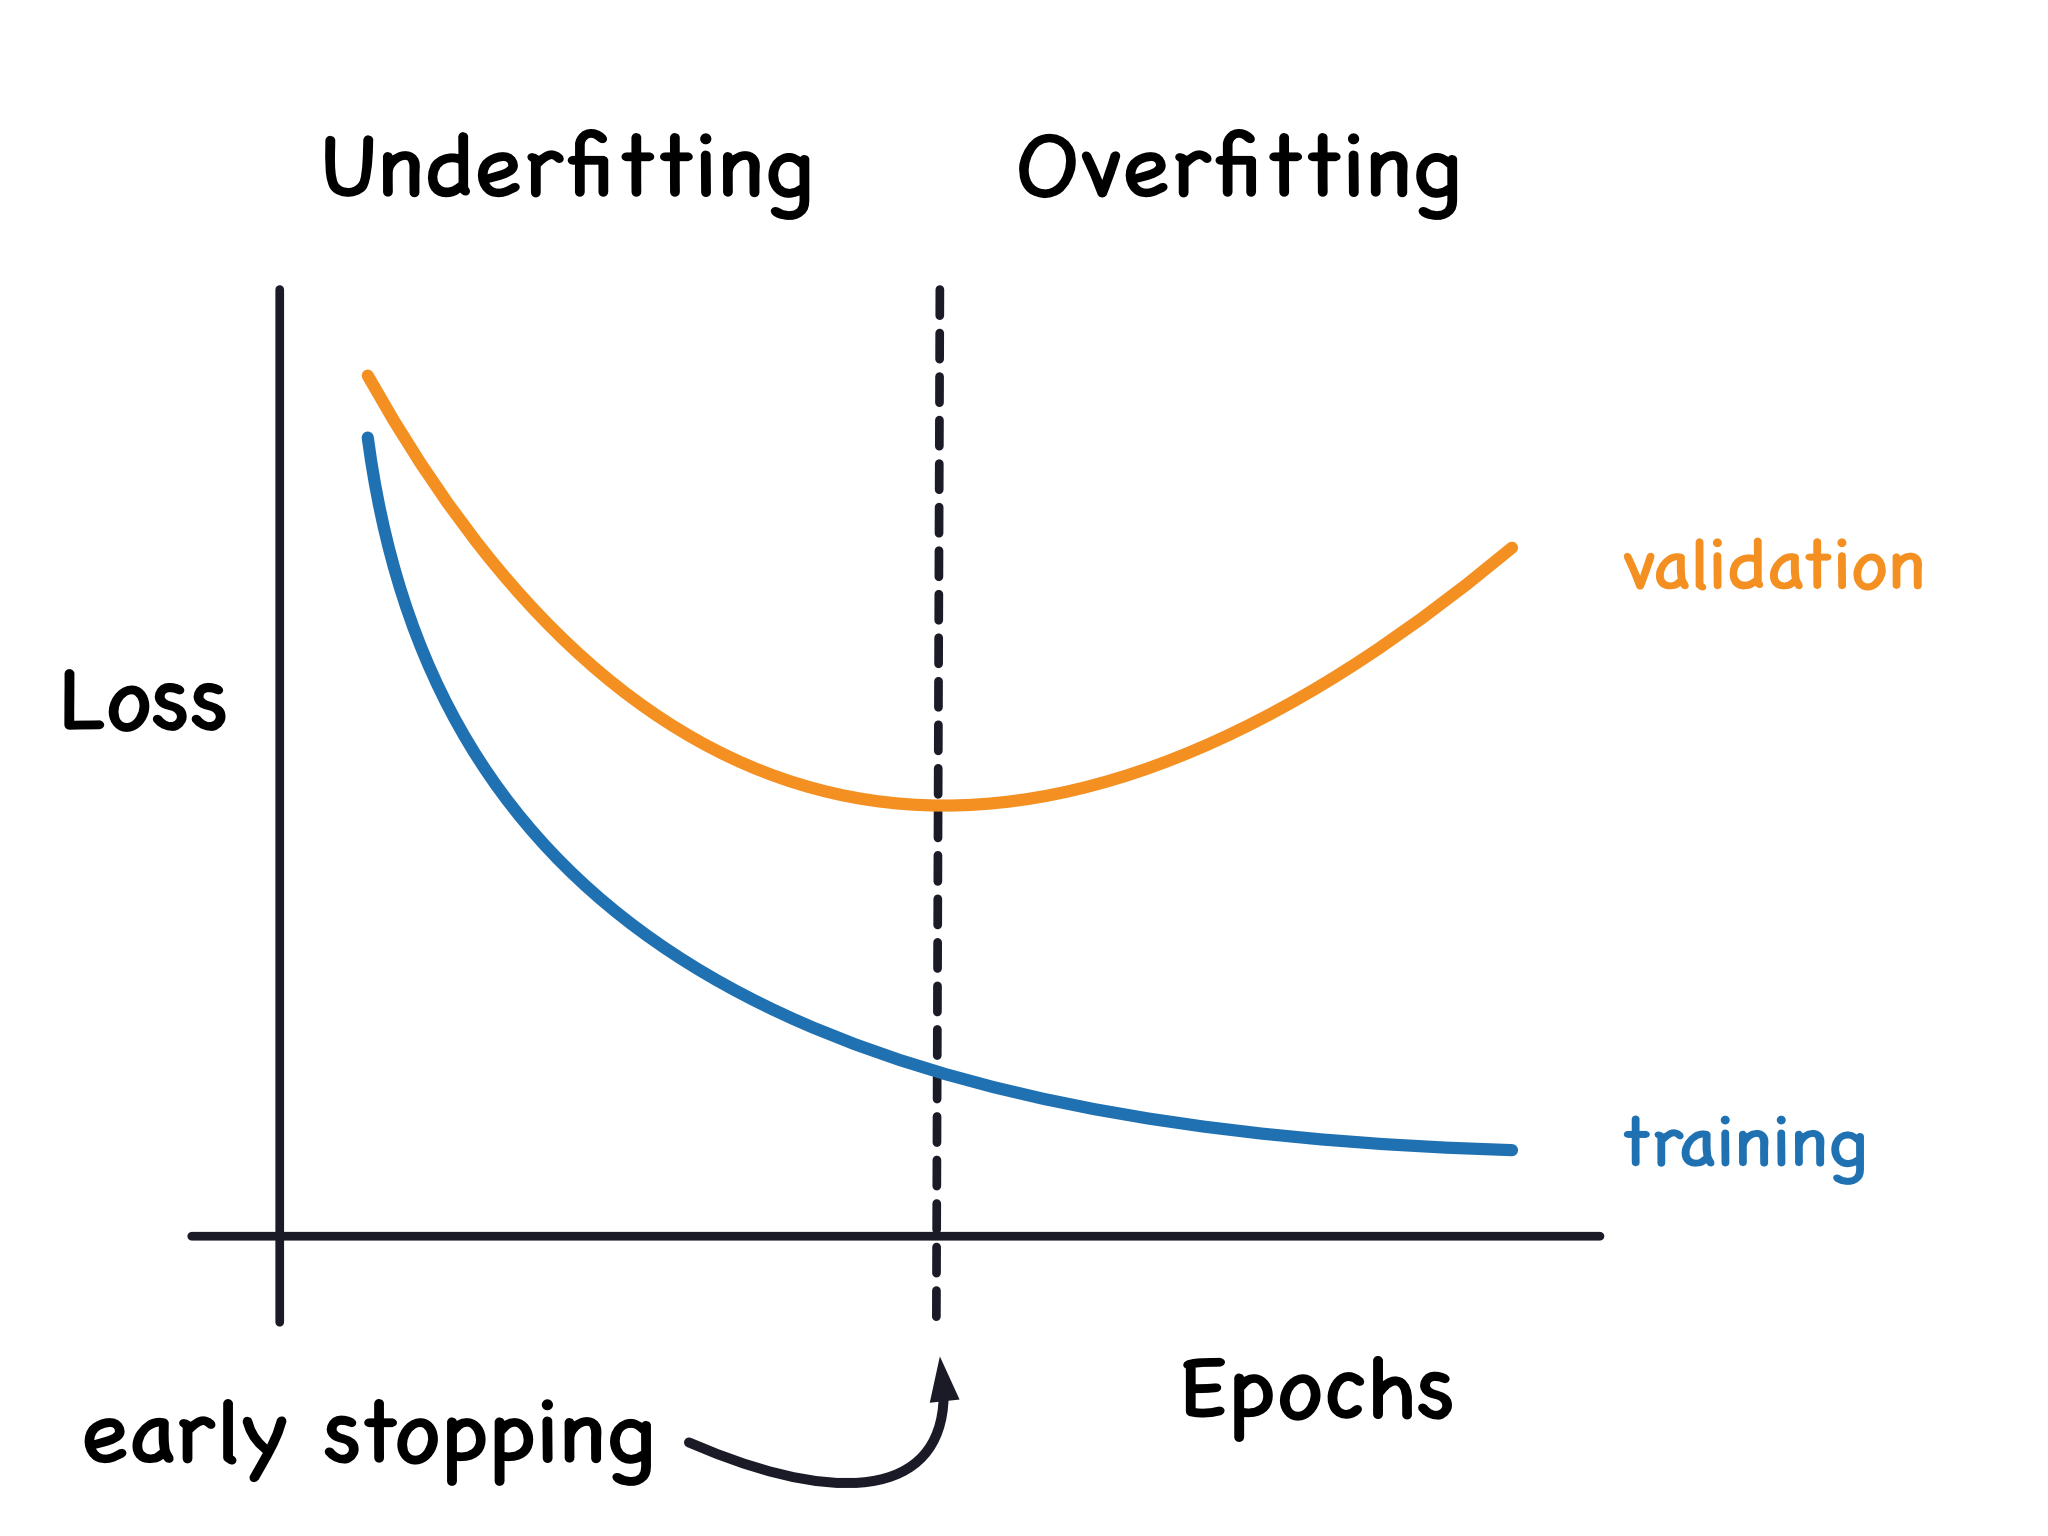
\includegraphics[width=0.45\textwidth]{pic/Early-Stopping.png}
                 \caption{\href{https://www.kaggle.com/code/ryanholbrook/overfitting-and-underfitting}{\textcolor{orange}{\textbf{Source}}}}
                \label{fig:Early-Stopping}
            \end{figure}
            
    \end{itemize}
\end{frame}

\begin{frame}{Key Regularization Techniques}
\begin{itemize}
    \item Dropout
    \begin{itemize}
            \item Randomly deactivates some of the neurons \textbf{during training}.
            \item Reduces neuron dependency and co-adaptation, thereby helping to prevent overfitting.
    \end{itemize}
    \end{itemize}
                \begin{figure}
            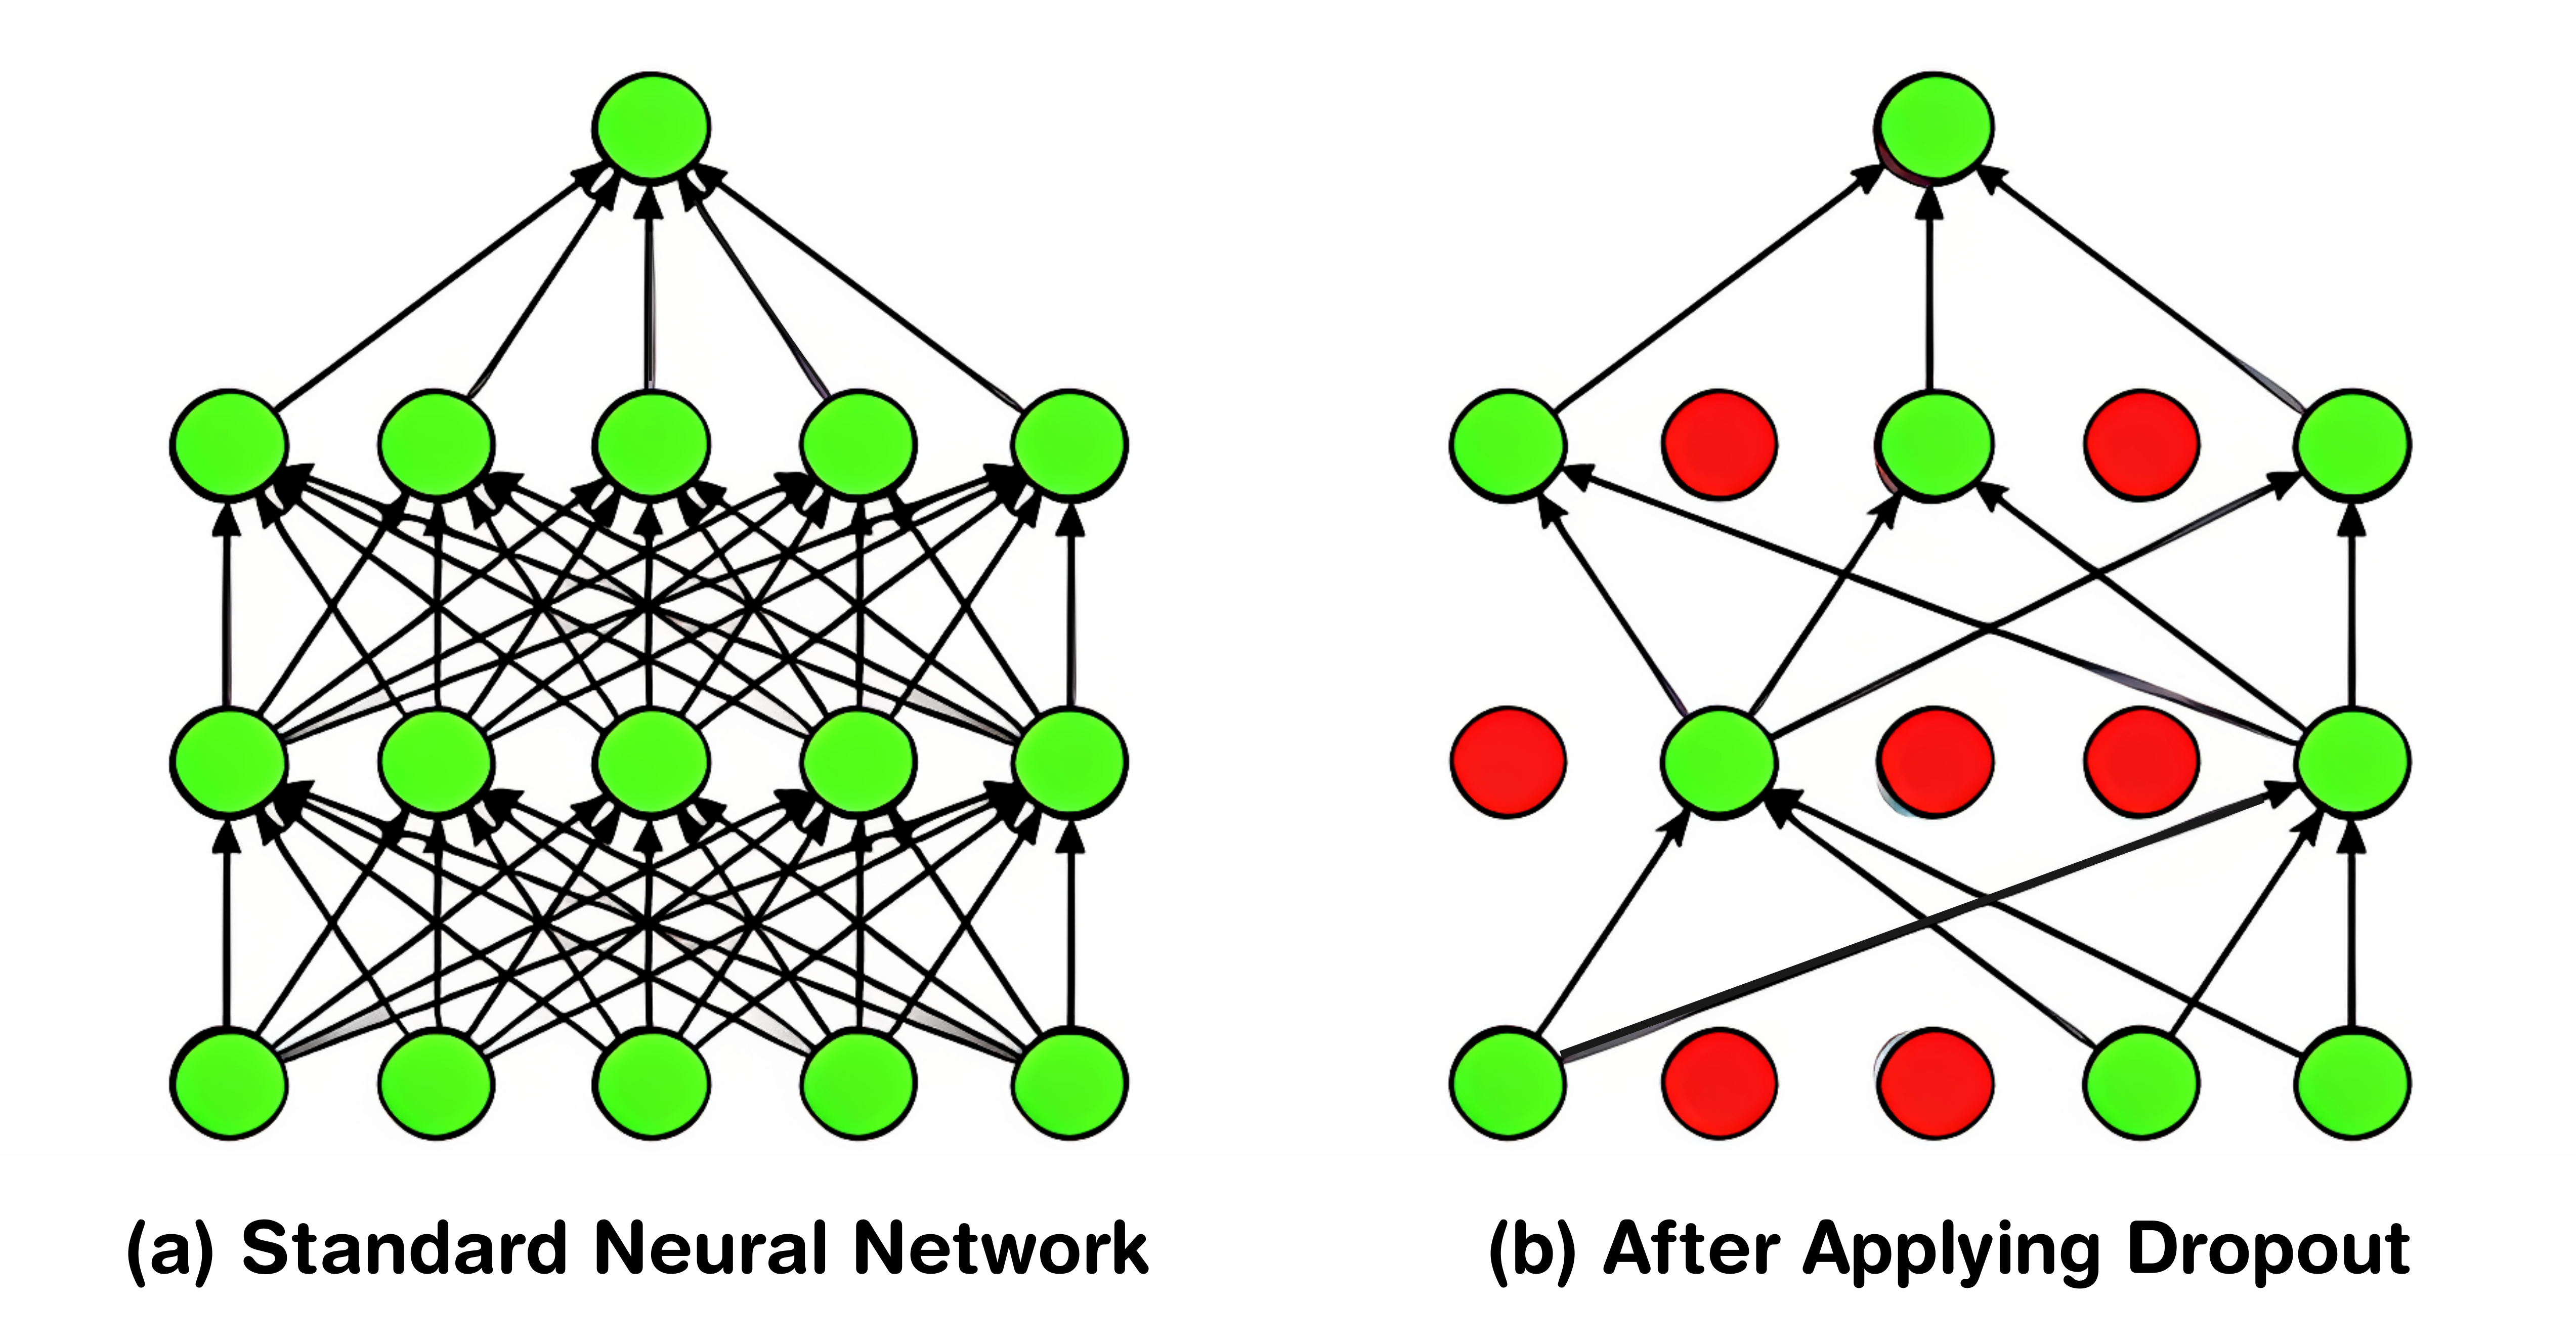
\includegraphics[width=0.55\textwidth]{pic/Dropout.png}
            \label{fig:Dropout}
        \caption{\href{https://miro.medium.com/v2/resize:fit:640/format:webp/0*EY8R7nS10y5kQzOx}{\textcolor{orange}{\textbf{Source}}}}
        \end{figure}

\end{frame}

\begin{frame}{Mechanism of Dropout}
    \begin{itemize}
        \item \textbf{During Training}
            \begin{itemize}
                \item A fraction (e.g., 20\%-50\%) of neurons in each layer is randomly set to zero during each forward pass.
                \item This fraction is called the \texttt{dropout rate}.
                \item The \texttt{dropout rate} is a value between 0 and 1. For example, if 30\% of neurons are deactivated, the \texttt{dropout rate} equals 0.3.
                \item Neurons are dropped out independently, and their weights are not updated during backpropagation.
            \end{itemize}
        \item \textbf{During Inference}
            \begin{itemize}
                \item All neurons are active.
                \item But the final weights will be larger than expected!
            \end{itemize}
    \end{itemize}
\end{frame}

\begin{frame}{Mechanism of Dropout}
    \begin{itemize} [<+-| alert@+>] % stepwise alerts
        \item<1-> \textbf{Challenge}
            \begin{itemize}
                \item<1-> During training, the network learns with a subset of neurons, leading to different activation patterns.
                \item<1-> During inference, when all neurons are active, the network’s learned weights might cause activations to differ from training due to the sudden increase in neuron count.
            \end{itemize}
        \item<2-> \textbf{Solution}
            \begin{itemize}
                \item The activations of all neurons during inference will be multiplied by \texttt{dropout rate}. This adjustment maintains the expected sum of activations, allowing the model to make predictions \textcolor{green}{comparable} to those during training.
            \end{itemize}
    \end{itemize}
\end{frame}

\begin{frame}{Why is Dropout a Good Regularization Idea?}
    \begin{itemize}
        \item \textbf{Prevents Overfitting} 
        \begin{itemize}
            \item Dropout forces the network to learn more robust features by preventing over-reliance on specific neurons.
            \item Randomly deactivating neurons during training reduces the risk of overfitting the training data.
        \end{itemize}

        \item \textbf{Acts as an Ensemble}
        \begin{itemize}
            \item Dropout effectively trains an ensemble of different sub-networks by sampling different neuron combinations in each iteration.
            \item During inference, these sub-networks are combined, resulting in a more generalized model that performs better on unseen data.
        \end{itemize}
    \end{itemize}
\end{frame}


\begin{frame}{Dropout Best Practices}
    \begin{itemize}
        \item \textbf{Dropout Rate:} Typically 0.5 for hidden layers, but it should be tuned based on the network architecture and problem complexity.
        \item \textbf{Where to Apply:} Commonly used in fully connected layers. For \textcolor{red}{convolutional layers} (discussed in the next chapter), spatial dropout is often preferred.
        \item \textbf{Use Sparingly:} Excessive dropout can cause underfitting or overly sparse networks.
    \end{itemize}
\end{frame}



\section{Training Improvements}
% \subsection{Activation Functions}

% \begin{frame}{Activation Functions}
%     \begin{itemize}
%     \item \textbf{Purpose:} Add non-linearity to the network.
%     \item \textbf{Intuition:} Activation functions decide if a neuron should "fire" based on its input, similar to how the brain responds to stimuli.
%     \end{itemize}
% \end{frame}


% \begin{frame}{Activation Functions}
%     \begin{itemize}
%         \item Choosing the right activation function based on the problem.
%         \item Effects on vanishing/exploding gradients.
%         \item Overview of common functions: ReLU, Sigmoid, Tanh, etc.
%     \end{itemize}
% \end{frame}


% \begin{frame}{Different Types of Activation Functions (Part 1)}
%     \centering
%     % \begin{tabular}{|c|c|c|}
%     % \centering
%     \begin{tabular}{|>{\centering\arraybackslash}m{4cm}|>{\centering\arraybackslash}m{5cm}|>{\centering\arraybackslash}m{4cm}|}
%         \hline
%         \textbf{Activation Function} & \textbf{Equation} & \textbf{Plot} \\
%         \hline
%         \textbf{Binary Step} &
%         $\text{Binary Step}(x) = \begin{cases}
%             1 & \text{if } x \geq 0 \\
%             0 & \text{if } x < 0
%         \end{cases}$ &
%         \begin{tikzpicture}[scale=0.35]
%             \begin{axis}[
%                 axis lines=middle,
%                 xlabel={$x$},
%                 ylabel={Binary Step$(x)$},
%                 ymin=-0.5, ymax=1.5,
%                 xmin=-2, xmax=2,
%                 samples=2,
%                 grid=both,
%                 width=6cm,
%                 height=6cm,
%                 ]
%                 \addplot[blue, thick, mark=*] coordinates {(-6, 0) (-0.01, 0) (0, 1) (6, 1)};
%             \end{axis}
%         \end{tikzpicture} \\
%         \hline

%         \textbf{Sigmoid} &
%         $\sigma(x) = \frac{1}{1 + e^{-x}}$ &
%         \begin{tikzpicture}[scale=0.3]
%             \begin{axis}[
%                 axis lines=middle,
%                 xlabel={$x$},
%                 ylabel={$\sigma(x)$},
%                 ymin=-0.1, ymax=1.1,
%                 xmin=-6, xmax=6,
%                 samples=100,
%                 domain=-6:6,
%                 grid=both,
%                 ]
%                 \addplot[green, thick] {1/(1 + exp(-x))};
%             \end{axis}
%         \end{tikzpicture} \\
%         \hline

%         \textbf{Tanh} &
%         $\tanh(x) = \frac{e^x - e^{-x}}{e^x + e^{-x}}$ &
%         \begin{tikzpicture}[scale=0.3]
%             \begin{axis}[
%                 axis lines=middle,
%                 xlabel={$x$},
%                 ylabel={$\tanh(x)$},
%                 ymin=-1.1, ymax=1.1,
%                 xmin=-6, xmax=6,
%                 samples=100,
%                 grid=both,
%                 ]
%                 \addplot[red, thick] {tanh(x)};
%             \end{axis}
%         \end{tikzpicture} \\
%         \hline

%     \end{tabular}
% \end{frame}

% % Second Frame
% \begin{frame}{Different Types of Activation Functions (Part 2)}
%     \centering
%     \begin{tabular}{|>{\centering\arraybackslash}m{4cm}|>{\centering\arraybackslash}m{5cm}|>{\centering\arraybackslash}m{4cm}|}
%         \hline
%         \textbf{Activation Function} & \textbf{Equation} & \textbf{Plot} \\
%         \hline

%         \textbf{ReLU} &
%         $\text{ReLU}(x) = \max(0, x)$ &
%         \begin{tikzpicture}[scale=0.3]
%             \begin{axis}[
%                 axis lines=middle,
%                 xlabel={$x$},
%                 ylabel={ReLU$(x)$},
%                 ymin=-1, ymax=6,
%                 xmin=-6, xmax=6,
%                 samples=100,
%                 grid=both,
%                 ]
%                 \addplot[cyan, thick] {max(0, x)};
%             \end{axis}
%         \end{tikzpicture} \\
%         \hline

%         \textbf{Leaky ReLU} &
%         $\text{Leaky ReLU}(x) = \begin{cases}
%             x & \text{if } x > 0 \\
%             \alpha x & \text{if } x \leq 0
%         \end{cases}$ &
%         \begin{tikzpicture}[scale=0.3]
%             \begin{axis}[
%                 axis lines=middle,
%                 xlabel={$x$},
%                 ylabel={Leaky ReLU$(x)$},
%                 ymin=-2, ymax=6,
%                 xmin=-6, xmax=6,
%                 samples=100,
%                 grid=both,
%                 ]
%                 \pgfmathsetmacro{\alpha}{0.1}
%                 \addplot[orange, thick] {x > 0 ? x : \alpha*x};
                
%             \end{axis}
%         \end{tikzpicture} \\
%         \hline

%         \textbf{ELU} &
%         $\text{ELU}(x) = \begin{cases}
%             x & \text{if } x > 0 \\
%             \alpha (e^x - 1) & \text{if } x \leq 0
%         \end{cases}$ &
%         \begin{tikzpicture}[scale=0.3]
%             \begin{axis}[
%                 axis lines=middle,
%                 xlabel={$x$},
%                 ylabel={ELU$(x)$},
%                 ymin=-2, ymax=6,
%                 xmin=-6, xmax=6,
%                 samples=100,
%                 grid=both,
%                 ]
%                 \addplot[purple, thick] {x > 0 ? x : 1*(exp(x) - 1)};
%             \end{axis}
%         \end{tikzpicture} \\
%         \hline

%     \end{tabular}
% \end{frame}

% \subsection{Weight Initialization}

% \begin{frame}{Key Initialization Techniques}
%     \begin{itemize}
%         \item \textbf{Zero Initialization:} Set all weights to zero (rarely used).
%         \item \textbf{Random Initialization:} Assign small random values to weights.
%         \item \textbf{Xavier Initialization:} Scales weights based on the number of neurons to maintain variance across layers.
%         \item \textbf{He Initialization:} Optimized for ReLU activation functions, scales weights to prevent vanishing/exploding gradients.
%         \item Prevent vanishing/exploding gradients with proper initialization.
%     \end{itemize}
% \end{frame}


\subsection{Hyperparameter Tuning}

\begin{frame}{Introduction to Hyperparameter Tuning}
    \begin{itemize}
        \item \textbf{Definition:} Hyperparameters are settings external to the model that control the training process and model capacity. They cannot be learned from the data.
        \item \textbf{Examples:} Learning rate, batch size, number of layers, number of neurons per layer, \textcolor{green}{dropout rate}, etc.
        \item \textbf{Impact:} Choosing the right hyperparameters can significantly enhance model performance, while poor choices may cause underfitting or overfitting.
    \end{itemize}
\end{frame}


\begin{frame}{Why Hyperparameter Tuning Matters}
    \begin{itemize}
        \item \textbf{Optimization Goal:} Identify the hyperparameters that maximize model performance on validation data.
        \item \textbf{Challenges:}
            \begin{itemize}
                \item Large, high-dimensional search space.
                \item High computational cost due to repeated training and evaluation.
                \item Noisy objective function – performance can vary due to randomness (e.g., weight initialization).
            \end{itemize}
        \item \textbf{Trade-offs:} Balancing computation time with model performance.
    \end{itemize}
\end{frame}


\begin{frame}{Approaches to Hyperparameter Tuning}
    \begin{itemize}
        \item \textbf{Grid Search:} An exhaustive search over a predefined set of hyperparameter combinations.
        \item \textbf{Random Search:} Randomly samples hyperparameters, sometimes finding good configurations more efficiently than grid search.
    \end{itemize}
    \begin{figure}
        \centering
        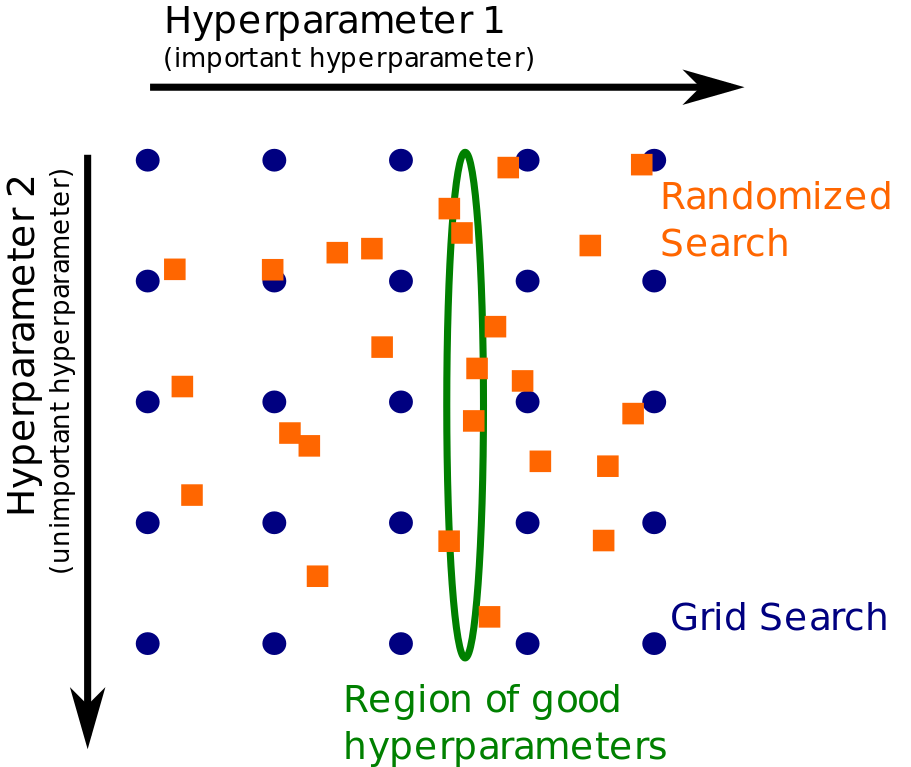
\includegraphics[width=0.3\textwidth]{pic/grid_vs_random_search.png}
        \caption{Grid Search vs. Random Search in Hyperparameter Tuning. \href{https://inria.github.io/scikit-learn-mooc/_images/grid_vs_random_search.svg}{\textcolor{orange}{\textbf{Source}}}}
        \label{fig:hyperparameter_tuning}
    \end{figure}
\end{frame}

\begin{frame}{Hyperparameter Tuning Best Practices}
    \begin{enumerate}
        \item \textbf{Start Simple:} Start by tuning a smaller subset of key hyperparameters (e.g., learning rate, batch size).
        \item \textbf{Use Cross-Validation:} Instead of a single validation set, use techniques like k-fold cross-validation to ensure performance is not dependent on a specific train-validation split.
        \item \textbf{Automate:} Leverage frameworks like \texttt{scikit-learn} to automate and parallelize the tuning process.
    \end{enumerate}
\end{frame}

\begin{frame}{Hyperparameter Tuning Best Practices}
    \begin{enumerate}
        \setcounter{enumi}{3}
        \item \textbf{Track Experiments:} Use tools like \texttt{Wandb} to systematically track hyperparameters, training metrics, and results.
        \item \textbf{Use Learning Curves:} Plot learning curves to monitor the model's performance over time and detect overfitting or underfitting early.
        \item \textbf{Budget Time and Resources:} Set limits on tuning (e.g., time, number of iterations) to avoid excessive computational costs.
    \end{enumerate}
\end{frame}



\subsection{Monitoring Training Process}

\begin{frame}{Monitoring Training Process}
    \begin{itemize}
        \item Track key metrics: Loss, accuracy, validation loss.
        \item Use \texttt{wandb} for real-time monitoring and logging.
        \item Wandb Panels: visualizations to explore your logged data, the relationships between hyperparameters and output metrics, and dataset examples.
        \item Detect overfitting early by analyzing trends in training and validation metrics.
        \item Visualize progress using learning curves to assess model performance over time.
    \end{itemize}
    \begin{figure}
        \centering
        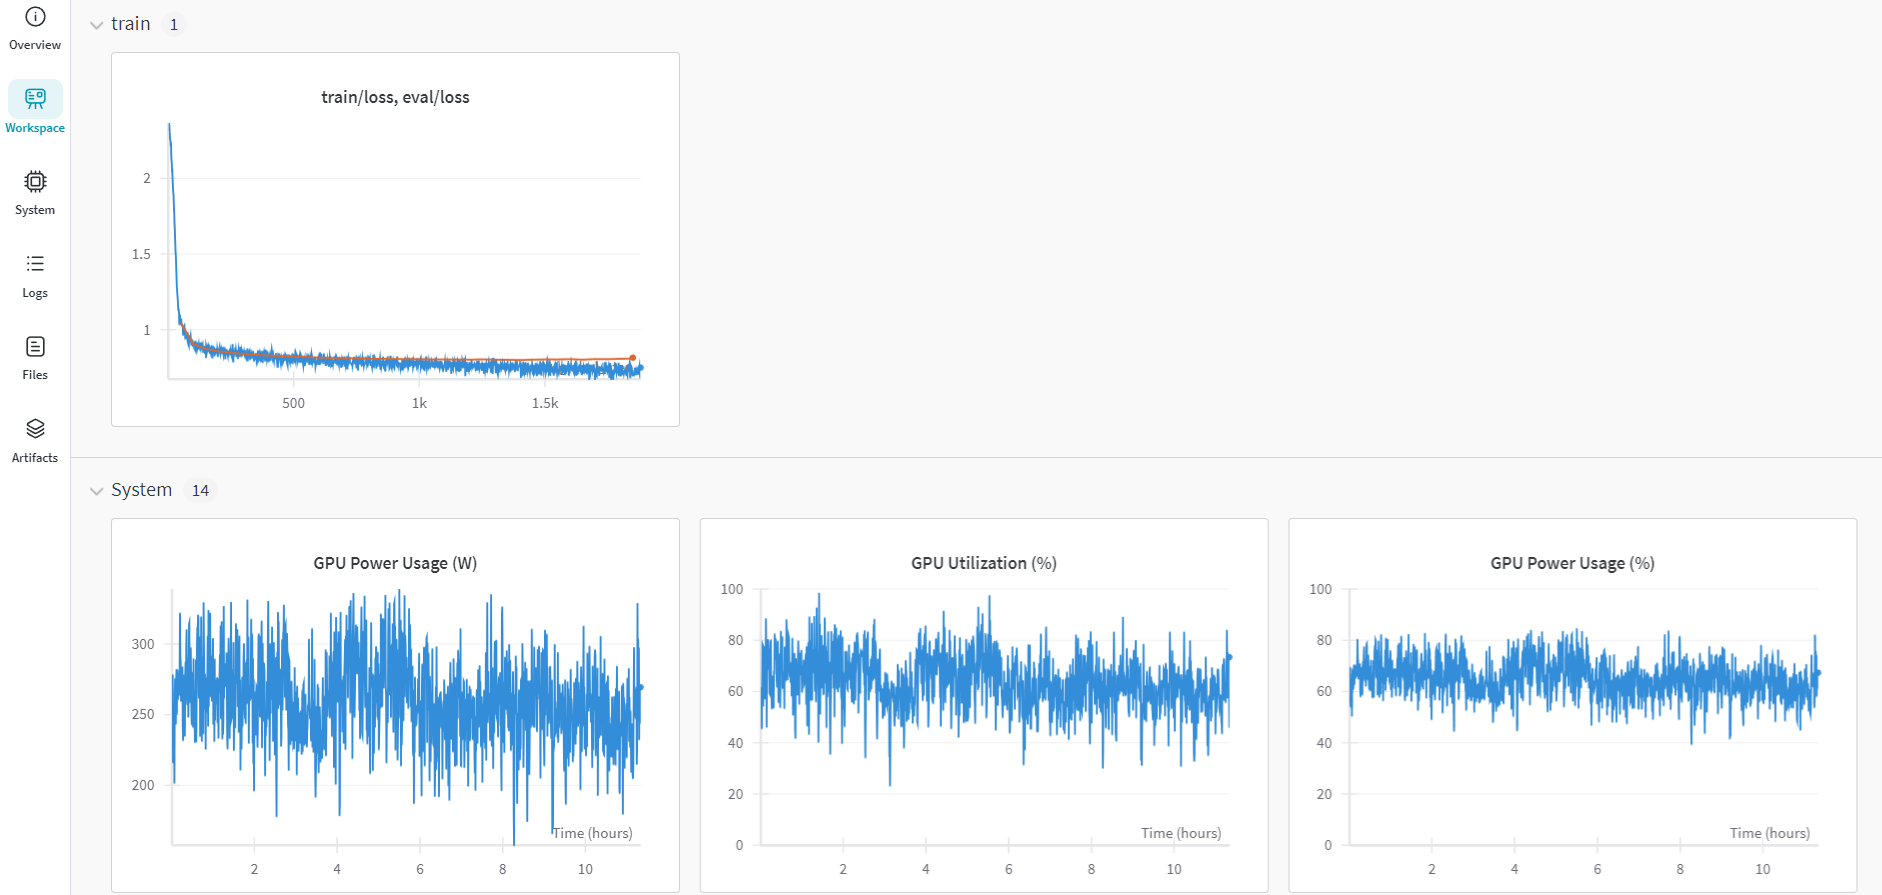
\includegraphics[width=0.5\textwidth]{pic/wandb.png}
        \caption{Training metrics visualization in \texttt{wandb}.}
        \label{fig:wandb}
    \end{figure}
\end{frame}



% \section{Batch Normalization}
% \subsection{Why Batch Normalization?}
% \subsection{How Batch Normalization Works}
% \subsection{Advantages and Disadvantages of Batch Normalization}
% \subsection{Batch Normalization in Practice}
% \subsection{Closing Takeaways on Batch Normalization}


\section{References}

\begin{frame}[allowframebreaks]
    \bibliography{ref}
    \bibliographystyle{ieeetr}
    \nocite{*} % used here because no citation happens in slides
    % if there are too many try use:
    % \tiny\bibliographystyle{alpha}
\end{frame}


\begin{frame}
    \begin{center}
        {\Huge Any Questions?}
    \end{center}
\end{frame}

\end{document}